\documentclass[12pt]{article}

\usepackage{wordlike}
\usepackage[backend=biber, maxbibnames=9]{biblatex}
\usepackage{amsmath, amsthm}
\usepackage{amssymb}
\usepackage{listings}
\usepackage[svgnames]{xcolor}
\usepackage{tikz}
\usepackage{array}
\usepackage{graphicx}
\usepackage{algpseudocode}
\usepackage{algorithm}
\usepackage{mathtools}
\usepackage{subcaption}
\usepackage{tabularx}
\usepackage{hyperref}

\addbibresource{ref.bib}
\graphicspath{ {./images/} }

\title{CAS 772 Final Project Report: Conjure - Controller-Free Hand Tracking for Computer Navigation}
\author{Anthony Hunt}

\begin{document}
\maketitle
\newpage

\section{Introduction}

% Controller-free hand-based navigation is common in modern VR/AR systems

Controller-free hand-based navigation remains one of the most marketable features of modern VR/AR systems. Manufacturers of VR hardware and software sell the promise of a user ``magically'' controlling their surroundings through simple, real world movements, with interactions that are much more flexible and intuitive than pushing buttons on a keyboard or moving the joystick of a controller. On a fundamental level, these products seem to dig at the instinctive desire to be understood by our surroundings with the complete spectrum of expression, rather than communicating with computers through pressing buttons or moving chunks of plastic.

As much as the quest for intuitive interactions is an HCI-oriented problem, there are a plethora of technical challenges that must be overcome before pushing these ideas from tech-enthusiast products into essential production systems. Some companies, like Apple, Samsung, and Meta, all have VR headsets that face these challenges head-on with high quality sensors, particularly for eye, head, and hand tracking. However, the hardware cost of these systems adds up quickly, requiring high-end on-device computing alongside expensive sensors and displays. In this project, we focus on finding the approximate limits of incorporating VR-like gestures into hardware most people already own.

We restrict ourselves to the following hardware: an iPhone with FaceID (although any phone with a depth/LiDAR sensor would work just as well), a USB cable, and a computer. With these tools, we attempt to enable gestures that translate hand movements into mouse cursor movements with a reasonable amount of latency. For the sake of this project, we consider a reasonable upper-latency limit to be 100 ms, although a recent survey \cite{latency} suggests 30-85 ms as a more appropriate modern target. In the 90s and early 2000s, a latency of 100 ms was considered the lower bound goal, however recent experiments (as summarized in \cite{latency}) state that a visual latency of even 11 ms is perceptible to the user. Beyond 100-150 ms, the perceived quality of human-machine interactions drastically decreased.

\section{Architecture}

The essential sensors for this project are those found on every modern iPhone: the RGB front-facing camera to stream colour video of the user and the TrueDepth camera used for FaceID to gather depth information relative to the phone's surface. An application collects these two streams of data, and by USB, sends them to the computer. On the computer side, a server-like application runs a thread to receive streamed video frames and another thread to process received frames. In the second thread, RGB images are passed through Google's Mediapipe Hand Landmarking and Gesture Recognition model \cite{mediapipe}. Then, smoothed depth values are appended to the resulting joint keypoints. Finally, computer control actions using PyAutoGUI are activated based on gesture classification and differences in the landmarks over time. The high-level view of the system is given by Figure~\ref{fig:highLevel}.

The mental model of the complete user+machine system is given by Figure~\ref{fig:mentalModel}. Generally, the phone will be propped up on a desk with the front-facing camera angled towards the user. Then, the user will wave their hands around within the phone's frame of view. There are two virtual depth-planes that mark depth-related cutoff points; the movement plane only tracks hand movements when the hand is in front of the plane (i.e. the hand is closer to the phone than some cutoff point) and the closer click-through plane only performs an action once the hand is in front of that plane. The RGB and depth streams are sent to the computer to perform actions as in Figure~\ref{fig:leftClickExample}. It is worth noting that the depth planes are projected in parallel to the touch-surface of the phone: Apple's TrueDepth sensor gives depth values as if they were orthographically projected on the touch-surface phone plane.

\begin{figure}
    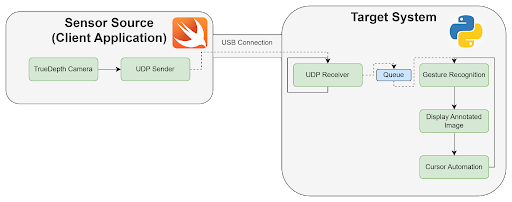
\includegraphics[width=0.8\textwidth]{highLevelArch}
    \centering
    \caption{High-level system architecture. Video data is transferred along the USB cable from the client/iPhone to the server/computer. The computer uses one thread to receive data and another to process data for actionable use.}
    \label{fig:highLevel}
\end{figure}

\begin{figure}
    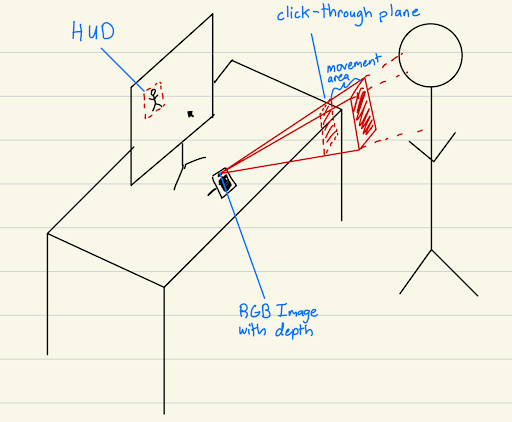
\includegraphics[width=0.5\textwidth]{mentalModel}
    \centering
    \caption{User and machine mental model. The user stands in front of the phone, making gestures around the two depth planes. The phone transfers data to the computer, which provides real-time feedback and takes action based on the gesture input.}
    \label{fig:mentalModel}
\end{figure}

\begin{figure}
    \begin{subfigure}[t]{0.32\textwidth}
    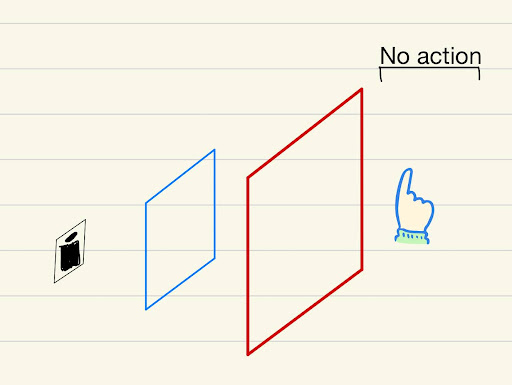
\includegraphics[width=\textwidth]{index_back}
    \caption{Hand is farther from the phone than the movement plane cutoff - no action.}
    \end{subfigure}
    \begin{subfigure}[t]{0.32\textwidth}
    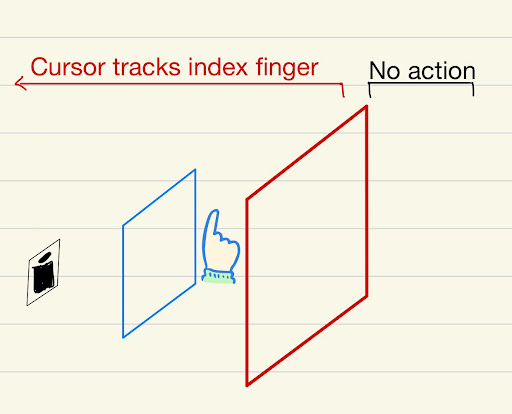
\includegraphics[width=\textwidth]{index_middle}
    \caption{Hand is in front of the movement plane but behind the click-through plane. The mouse cursor matches hand movements exactly (specifically, it tracks the tip of the index finger).}
    \end{subfigure}
    \begin{subfigure}[t]{0.32\textwidth}
    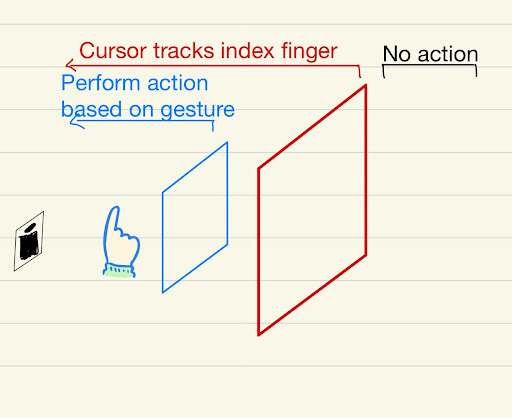
\includegraphics[width=\textwidth]{index_front}
    \caption{Hand is in front of the click-through plane. The computer automation performs a ``mouse left-click'' action.}
    \end{subfigure}
    \centering
    \caption{Depth plane impact when moving a hand with the ``pointing index finger'' gesture.}
    \label{fig:leftClickExample}
\end{figure}

\subsection{The Data Transfer Protocol}
Over the course of this project, I tested 5 unique data transfer protocols to find the one most suitable for hand tracking computer vision. The main payload of this system is two streams of 640x480p video: one stream of 3-channel 8-bit RGB, and another for 16-bit floating depth values. The resolution choice is largely decided for us by Apple's AVFoundations library, since the TrueDepth camera only works with specific (low) resolutions. The criteria for a suitable data transfer protocol is:
\begin{itemize}
    \item Data on the receiver end must be clear. Some lossy video compression codecs (like H264) can leave smearing, blurring, and compression artifacts on the video decoded by the receiver. This is a non-starter for machine learning tasks, as edges between the hand and background must be clearly defined.
    \item The stream of data must have adequate throughput. Although the video we are sending only has a resolution of 640x480p, each uncompressed frame of video is around 1.15MB. If too many of these frames are dropped, the video can look incredibly choppy and unnatural. Movements may not translate appropriately into computer actions.
    \item The stream of data must have low latency (targeting $<50$ ms with a requirement of $<100$ ms, corresponding to 20 and 10 fps respectively). If the lag is too great, users will become disconnected with the computer's actions and feedback provided by the system on future actions will be useless. In our system, the computer control system is expected to be slower than the video streaming producer, so ideally, the server-side receiver will only need to process the most recent available frame.
\end{itemize}

For the interim presentation, I attempted to use plain WebRTC \cite{webrtc} over WiFi to transfer data. WebRTC is a real time communications library for JavaScript, historically preferred for real time video streaming. With a little bit of setup and digging for the community-made Swift bindings, I was able to get a somewhat-stable video stream working between my phone and computer. However, passing WebRTC video streams into a machine learning system proved to be very difficult to work with. Among the problems related to setting up the initial connection (which could be resolved through additional external tools like Tailscale and a small custom HTTP server), received WebRTC video often contained heavy compression artifacts, smearing, inconsistent resolutions, and very high latency, even on high-speed networks. Afterwards, I experimented with running WebRTC through a USB cable by mocking an ethernet connection between my phone and computer, but WebRTC both preferred to use WiFi even when physically connected and seemed to arbitrarily limit the throughput of data even when running over USB. Struggles were further compounded by sparse documentation,  undocumented API differences between the official JavaScript and Swift bindings, and slow conversion of depth images to a corresponding colour map (I even tried to create a Metal shader at one point!).

After the presentation, I set up Mediapipe to run hand tracking inference locally on the phone. The initial hope was that reducing the payload from two video streams to 21 keypoints would cut down on the latency seen when using WebRTC.
At first, I gave up on the on-device solution since I was getting very poor frame rates ($<3$ fps) and general unresponsiveness. However, experimenting with the timings revealed a critical timestamped-based bug of my own making causing an extra around 1-second delay to each processed frame. Once fixed, on-device Mediapipe gave reasonable latency (around 42-60 ms when measured using print statements) and felt responsive enough to work with in practice.

Since the phone would be stationary for the duration of use, I switched my focus to creating a simple, custom transport protocol over USB. In my previous experiments, I found that compression and latency were both make-or-break features of making video streaming feel natural and usable, so I tried to limit the amount of CPU work on the phone side. Although TCP isn't the most fitting tool for real-time video streaming, rolling out TCP packets with raw, uncompressed frame data was extremely simple. Testing with this protocol seemed to perform surprisingly well, with zero compression artifacts and a reasonable frame rate. We note that USB 2.0 has a maximum practical data transfer rate of 30-40MB/s, so a reliable 20-30 fps was more than achievable. However, since TCP guarantees delivery, the protocol enforces that all frames must be processed by the receiver. This behaviour in turn means that our slightly-slower Python USB receiver thread would fall increasingly out of sync with real world interactions as unread frames accumulated over time.

Logically, my next step was to replace TCP with UDP. This process was relatively painless, since we only needed to add in packet-splitting on the producer device and packet-combining on the receiver end. From rudimentary testing, 9000 byte datagram sizes seemed to perform well enough for this project. Although UDP over USB sometimes fails on MacOS, it had very low latency (50 ms) and high quality video streaming on my Windows system.

Mediapipe states \cite{mediapipe} that its CPU inference latency is about 16.7 ms (on an unspecified CPU). In practice, on my Intel i7-14700k, I saw a median of 15 ms per frame with spikes to 30 ms per frame about 10\% of the time. With on-device Mediapipe, the inference latency jumped to 42-60 ms. Oddly enough, the image annotation and displaying method (opencv-python) used in my Python script caused the most delay at around 200 ms per frame. This distribution of latency implies that massive performance improvements could be gained by choosing a more streamlined video streaming and annotation library.

\subsection{Hand Landmarking and Automation Actions}

Once we found a reliable stream of data, the RGB video frames could be passed to the Mediapipe landmarking model. We note that the model used in Conjure is not the default model provided by Google, but one that was fine-tuned to accept a different set of classifications, closer to the gestures used in VR systems. For example, the default model does not have a pinch-like gesture, but the fine-tuned model does. As a disclaimer, the actual fine-tuning of the model was completed for a different project in my undergrad, but Mediapipe provides APIs that make the process completely painless. For the extra gesture classifications, I selected 11 from the HAGRID hand gesture dataset \cite{hagridV22024}. Of these, the most relevant are pointing with an index finger (``one''), a peace sign, pointing with the index and middle fingers (``two-up''), and showing an open palm (``palm'' or ``stop'') - see Figure~\ref{fig:gestures}.

\begin{figure}
    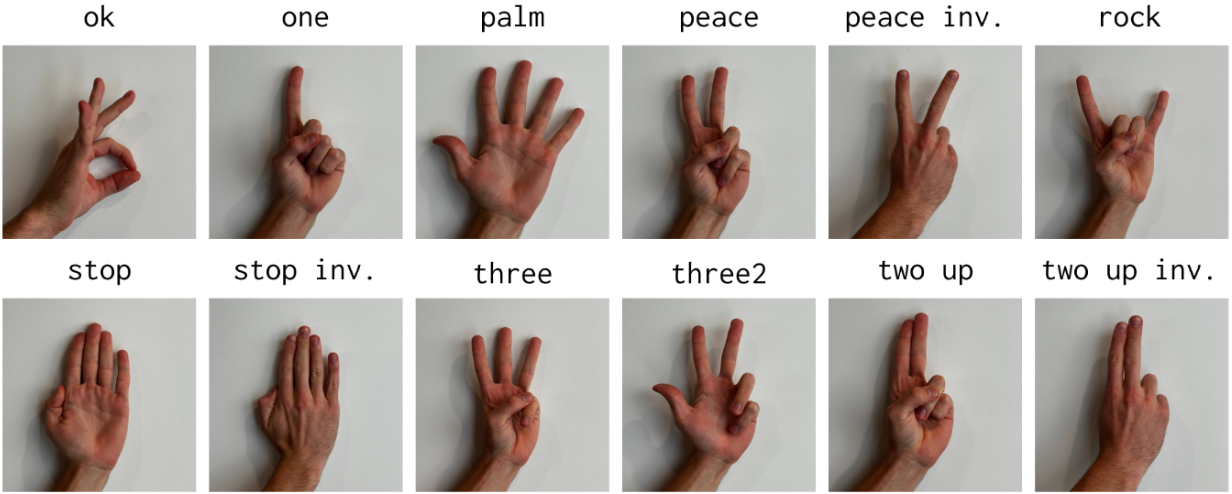
\includegraphics[width=\textwidth]{hagrid_hands}
    \caption{Example hand gestures provided by the HAGRID dataset.}
    \label{fig:gestures}
\end{figure}

After the landmarks and classification are returned, we attach the minimum of the 9 nearest depth pixels to each keypoint, determined by closeness in the x-y camera projection pixels. Feedback on depth information is provided to the user through an annotated video stream: the movement plane projects a grid of circles that become brighter as the user approaches the depth plane. Once past, the circles become white. The click-through plane uses a similar technique, but only annotates circles on the tips of each finger, glowing bright blue once the threshold has been passed. Figure~\ref{fig:depthMap} contains an example image.

\textit{Note}: After my initial submission, I experimented with on-device Mediapipe a little more. Since we do not get image data from this method, the resulting feedback just plots the dots on a black background, as in Figure~\ref{fig:depthMapOnDevice}

\begin{figure}
    \begin{subfigure}[t]{0.32\textwidth}
    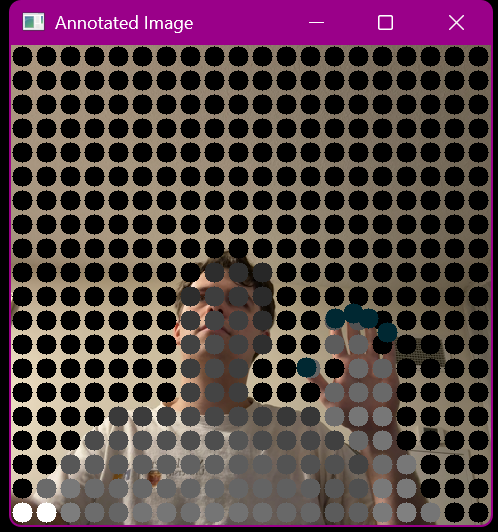
\includegraphics[width=\textwidth]{hand_back}
        \caption{Hand is behind both planes.}
    \end{subfigure}
    \begin{subfigure}[t]{0.32\textwidth}
    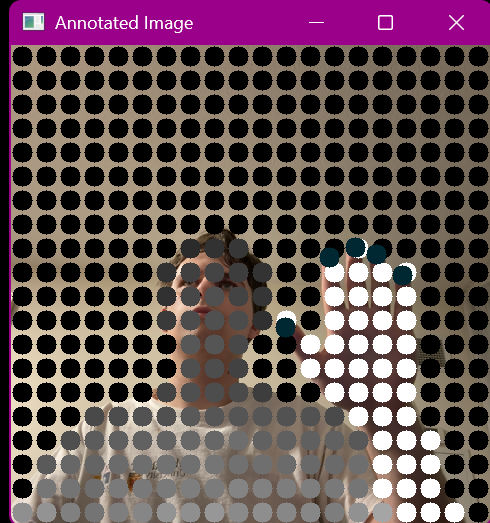
\includegraphics[width=\textwidth]{hand_middle}
        \caption{Hand is in front of the movement plane.}
    \end{subfigure}
    \begin{subfigure}[t]{0.32\textwidth}
    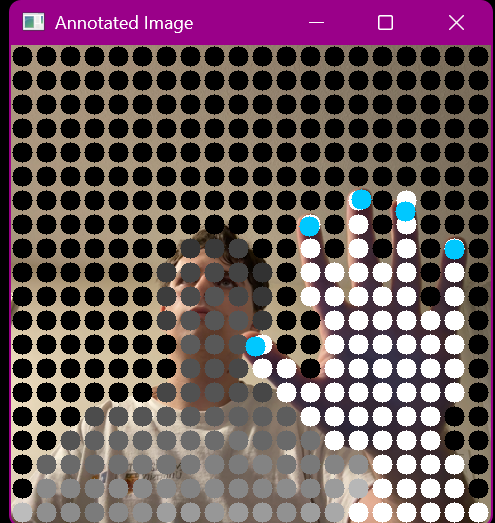
\includegraphics[width=\textwidth]{hand_front}
        \caption{Hand is in front of the click-through and movement plane.}
    \end{subfigure}
    \centering
    \caption{RGB image annotated with depth information. When the grid of black dots turns white, the user has passed the movement plane. When the dots on fingers turns blue, they have passed through the click-through plane.}
    \label{fig:depthMap}
\end{figure}
\begin{figure}
    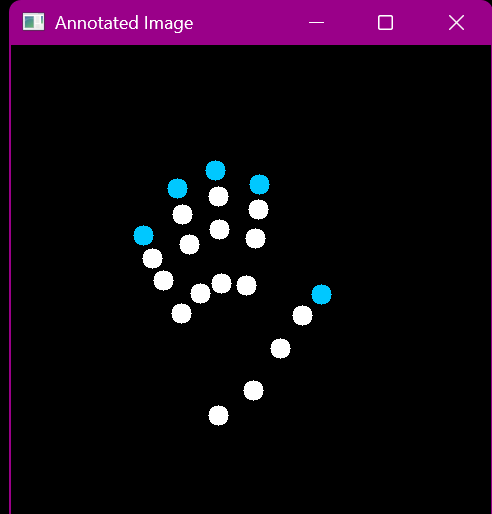
\includegraphics[width=0.32\textwidth]{hand_mediapipe}
    \centering
    \caption{Landmark-only projection (no image/depth image data available). Depth dots are projected on a black background but have the same effect as Figure~\ref{fig:depthMap}}
    \label{fig:depthMapOnDevice}
\end{figure}

Actions are then carried out by PyAutoGUI based on the following table:
\begin{table}[h!]
\centering
% \renewcommand{\arraystretch}{1.4}
\begin{tabularx}{\textwidth}{| l | X | X |}
\hline
\textbf{Area} & \textbf{Gesture} & \textbf{Action} \\
\hline
Anywhere & Palm / Stop & Stop all movement \\
\hline
Movement Plane & One (pointing with index finger) & Cursor tracks index finger movement precisely \\
& Two-up (pointing with index and middle finger) & Cursor follows index finger movement with decaying velocity \\
\hline
Click-through Plane & One & Mouse left-click \\
& Peace & Mouse right-click \\
& OK (pinch) & Mouse left-click and hold (for clicking+dragging)\\
\hline
\end{tabularx}
\end{table}

\section{Conclusion}

Conjure is successful in its primary goal: creating a proof-of-concept system that can provide a glimpse of VR-like hand controllers on the computer at no cost. However, given the lack of time and subjects for user testing, along with my rudimentary knowledge of proper HCI-based development, some gestures are not as intuitive as I would have liked. For example, given the arbitrary placement of depth planes at some pre-determined depths, it is all too easy to accidentally pass through either of the planes unintentionally. At the same time, some ``click'' motions do not register because the user's hand may be just behind the click-through plane. Although I attempted to make the computer's actions more transparent through annotating the image stream with depth values, these controls still feel unrefined.

One way to mitigate such clunky depth plane interactions could be to define relative movement planes. That is, instead of arbitrarily-set constants for the plane depths, we could use the relative depth movement of the hand to determine when to perform a click or cursor movement. When a user's hand moves towards the camera, that signifies they wish to advance into the next plane. Likewise, when they move away from the camera, it is reasonable to assume they wish to leave the current plane. This movement would also reduce reliance on gesture-specific actions, since the movement controls would be more fine-grained and easier to work with.

In addition, some gestures do not work well compared to their VR origins. The pinch-to-drag-windows motion common in VR is tricker to implement than anticipated, requiring OS-specific implementations and a better mechanism for determining the start/stop gestures than is currently implemented. Velocity-enabled cursor movement could be useful, especially if the user wishes to move a long distance across multiple monitors, but the overly-sensitive depth planes and rigid gestures make the interaction feel less like gliding along a trackpad and more like herding a bug with a stick. All of these gestures can be improved through the HCI development process, gathering feedback from multiple subjects, using better signifiers of different modes (for example, velocity-enabled vs. positional-only movement), and increasing the cleverness of using the available data.

Further technical challenges still remain of course, least of all configuration settings, specific gestures, and per-person tuning, but this project demonstrates the core ideals of VR-like movement in everyday computing. Further improvements lie in processing feedback for the user and incorporating more depth-related information. For example, dragging a window from the foreground to the background, or interacting with objects in 3D in Blender or CAD. Since hand position, depth, and RGB video information are now freely available to computers, HCI surveying and experimentation are necessary to take this work to the next step, with the goal of providing truly intuitive and useful gestures.

Note: The source code is available at \url{https://github.com/Ant13731/conjure}.


% Notes addressing feedback:
% -/ get HCI reference for a reasonable amount of latency (maybe find the highest number of ms before a person notices lag)
% -x Address lack of codec options on WebRTC? I mean you can use VP8, VP9 and AV1 if it is supported, but we have better options to choose from...
% -/ profile mediapipe inferencing on server and on phone
% -/ depth pixels are all orthographically projected
% - Quantitative Evaluation
% -/ Limitations and main take-aways
%   -/ Difficult to determine planes physically

% Video script
% Show all basic gestures?


% EXPERIMENT ON-DEVICE MEDIAPIPE
% - ~42-60 ms of latency measured through print statements...

\pagebreak
% \nocite{*} % keeps all references, even those not referred to
\printbibliography
\end{document}